\chapter{استنتاج مورد کاربرد‌ها از نیازمندی‌‌ها}		
در این گام، استخراج مورد کاربرد‌ها از نیازمندی‌ها صورت گرفت و در ادامه، نمودار‌‌های مورد کاربرد‌ها، جدول بازبینی و جدول تخصیص موارد کاربرد به تکرار‌‌ها ترسیم شد. کنشگران این سیستم، کاربران در نقش‌های کارجو و کارفرما می‌باشند.

\section{شناسایی مورد کاربرد‌ها}		
در این مرحله از تعداد 26 نیازمندی شناسایی شده، 28 مورد کاربرد استنباط و شناسایی شد.

\section{تعیین قلمرو مورد کاربرد‌ها}		
لیست مورد کاربرد‌ها به صورت زیر است:
\begin{enumerate}
	\item[] \ucstep{ثبت‌نام کاربر:} 			
	
	\tuc				
	{کاربر بر روی پیوند ثبت‌نام در صفحه اصلی سایت کلیک می‌کند.}				
	{کاربر در صورت موفق‌آمیز بودن ثبت‌نام، وارد پنل کاربری می‌شود، در غیر این صورت به صفحه‌ی اصلی سایت هدایت می‌شود.}
	
	\item[] \ucstep{ورود به سامانه:} 			
	\tuc				
	{کاربر بر روی پیوند ورود به سامانه در صفحه اصلی سایت کلیک می‌کند.}				
	{کاربر پنل شخصی خود را مشاهده می‌کند.}
	
	\item[] \ucstep{خروج از سامانه:}
	\tuc				
	{کاربر به روی دکمه‌ی خروج در پنل کاربری کلیک می‌کند.}				
	{کاربر صفحه اصلی سایت را مشاهده می‌کند.}
	
	\item[] \ucstep{بازیابی رمزعبور فراموش شده:}
	\tuc				
	{کابر بر روی دکمه \say{بازیابی رمز عبور} در صفحه ورود سایت کلیک می‌کند.}				
	{کاربر پیامک حاوی رمز عبور موقت را دریافت می‌کند.}
	
	\item[] \ucstep{مشاهده‌ی پروفایل:}
	\tuc				
	{کاربر بر روی آواتار در پنل کاربری خودش کلیک می‌کند.}				
	{کاربر اطلاعات شخصی خود را در صفحه‌ی پروفایل مشاهده می‌کند.}
	
	\item[] \ucstep{آپدیت اطلاعات کاربری:}
	\tuc				
	{کابر بر روی پیوند \say{تغییر اطلاعات} در قسمت نوار ابزار پنل کاربری کلیک می‌کند.}	
	{کاربر پیغام \say{تغییر اطلاعات با موفقیت انجام شد.} را مشاهده می‌کند.}
	
	\item[] \ucstep{خرید اکانت پرمیوم:}
	\tuc				
	{کاربر به روی دکمه‌ی \say{خرید} در صفحه‌ی ارتقا اکانت کلیک می‌کند.}
	{کاربر پیغام \say{اکانت پرمیموم با موفقیت فعال شد} را مشاهده می‌کند.}
	
	\item[] \ucstep{ساخت رزومه:}
	\tuc				
	{کارجو به روی دکمه‌ی \say{ساخت رزومه} در صفحه‌ی پروفایل کاربری، در صحفه‌ی مربوط به کارجو، کلیک می‌کند.}
	{کارجو پیغام \say{روزمه ساخته شد} را مشاهده می‌کند.}
	
	\item[] \ucstep{مشاهده‌ آگهی‌های پیشنهادی:}
	\tuc				
	{کارجو بر روی علامت ذره‌بین (مخصوص دیدن آگهی‌ها مثل اکسپلور اینستاگرام) در صفحه‌ی اصلی کارتاپ کلیک می‌کند.}
	{کارجو آگهی‌ها را مشاهده می‌کند.}
	
	\item[] \ucstep{ذخیره ‌کردن آگهی:}
	\tuc				
	{کارجو بر روی دکمه‌ی \say{ذخیره کردن آگهی} در صفحه‌ی آگهی کلیک می‌کند.}				
	{کارجو پیغام \say{آگهی ذخیره‌ شد.} را مشاهده می‌کند.}
	
	\item[] \ucstep{مشاهده پروفایل کارجویان:}
	\tuc				
	{کارفرما به روی آواتار یا نام کاربری کارجو در صفحه‌ی پیشنهادات یا جستجو کلیک می‌کند.}				
	{کارفرما اطلاعات پروفایل کارجو را مشاهده می‌کند.}
	
	\item[] \ucstep{ارسال رزومه:}\label{uc:resume}
	\tuc				
	{کارجو بر روی دکمه \say{ارسال رزومه} در صفحه آگهی یک شرکت کلیک می‌کند.}
	{کارجو پیغام \say{پیغام رزومه ارسال شد.} یا پیغام \say{فرمت فایل ارسالی درست نیست، لطفا مجدداً تلاش کنید.} را مشاهده می‌کند.}
	
	\item[] \ucstep{مشاهده‌ی پروفایل شرکت‌‌ها:}\label{uc:company-profile}
	\tuc				
	{کاربر بر روی پروفایل یک شرکت در صفحه معرفی شرکت‌ها کلیک می‌کند.}				
	{کاربر اطلاعات مربوط به شرکت مدنظر را مشاهده می‌کند.}
	% --------------------------------------------------------
	\renewcommand{\labelenumi}{\alph{enumi})}
	% --------------------------------------------------------
	
	\item[] \ucstep{ثبت آگهی توسط کارفرما:}
	\tuc
	{کارفرما بر روی دکمه \say{ثبت آگهی} در پنل کاربری کارفرما کلیک می‌کند.}
	{کارفرما پیغام 
		\begin{enumerate}
			\item 
			آگهی با موفقیت ثبت شد.
			\item 
			پرداخت ناموفق بود، آگهی ثبت نشد.
		\end{enumerate} را مشاهده می‌کند.}
	% --------------------------------------------------------
	\renewcommand{\labelenumi}{\arabic{enumi})}
	% --------------------------------------------------------
	
	\item[] \ucstep{مشاهده کارجویان پیشنهادی:}
	\tuc
	{کارفرما بر روی گزینه \say{کارجویان پیشنهادی به شرکت شما} در پنل کاربری کارفرما کلیک می‌کند.}
	{کارفرما اطلاعات کارجویان پیشنهادی را مشاهده می‌کند.}
	
	\item[] \ucstep{احراز هویت}
	\tuc				
	{کاربر برروی دکمه‌ی ثبت درخواست آگهی در صفحه‌ی آگهی مربوطه و یا ثبت شرکت در صفحه‌ی اصلی سایت کلیک می‌کند.}			
	{کاربر پیامک تایید احراز هویت را دریافت می‌کند.}
	
	\item[] \ucstep{نشان‌دار کردن آگهی:}\label{uc:bookmark}
	\tuc
	{کارجو بر روی علامت ستاره در صفحه مربوط به آگهی مدنظر کلیک می‌کند.}
	{کارجو پیغام \say{آگهی به لیست آگهی‌های نشان‌دار افزوده شد} یا \say{آگهی‌ از نشان‌دار‌ها حذف شد.} را مشاهده می‌کند.}
	
	\item[] \ucstep{مشاهده‌ی وضعیت آگهی‌های درخواستی:}\label{uc:see-reqs}
	\tuc		
	{کارجو به روی دکمه‌ \say{وضعیت آگهی‌های درخواستی} در قسمت نوار ابزار پنل کاربری کارجو کلیک می‌کند.}
	{کارجو لیستی از آگهی‌ها و وضعیتشان را مشاهده می‌کند.}
	
	\item[] \ucstep{مشاهده درخواست همکاری کارفرماها:}
	\tuc		
	{کارجو به روی دکمه‌ \say{درخواست‌های همکاری} در قسمت نوار ابزار پنل کاربری کارجو کلیک می‌کند.}
	{کارجو لیستی از شغل‌های پیشنهاد شده از سمت کارفرماها را مشاهده می‌کند.}
		
	\item[] \ucstep{ارسال پیام دعوت به همکاری:}
	\tuc				
	{کارفرما بر روی دکمه \say{دعوت به همکاری} درصفحه کارجوی مدنظر کلیک می‌کند.}
	{کارفرما پیغام \say{پیام با موفقیت ارسال شد.} را مشاهده می‌کند.}
	
	\item[] \ucstep{مدیریت درخواست‌ها:}\label{uc:req-manage}
	\tuc				
	{کارفرما بر روی دکمه \say{مدیریت درخواست‌ها} در پنل کاربری کلیک می‌کند.}
	{کارفرما لیستی از درخواست‌های کارجویان را مشاهده می‌کند.}
	
	\item[] \ucstep{جستجوی آگهی‌ها:}\label{uc:apply-search}
	\tuc				
	{کاربر روی نوار جستجو در صفحه‌ی اصلی کلیک می‌کند.}
	{کاربر نتیجه جستجو را مشاهده می‌کند.}
	
	\item[] \ucstep{فیلتر آگهی‌ها:}
	\tuc				
	{کاربر بر روی گزینه فیلتر کلیک می‌کند.}
	{کاربر لیست آگهی‌های فیلتر شده را مشاهده می‌کند.}
	
	\item[] \ucstep{مشاهده رزومه‌ها:}\label{uc:see-resumes}
	\tuc				
	{کارفرما بر روی دکمه \say{رزومه} در صفحه پروفایل کارجوی مدنظر کلیک می‌کند.}
	{کارفرما یا رزومه را مشاهده کرده یا پیغام \say{عدم پیغام رزومه} را می‌بیند.}
	
	\item[] \ucstep{ثبت شرکت:}
	\tuc				
	{کارفرما بر روی دکمه \say{ثبت شرکت} در صفحه اصلی سایت کلیک می‌کند.}
	{کارفرما پیغام \say{شرکت شما با موفقیت ثبت شد.} را مشاهده می‌کند.}
	
	\item[] \ucstep{آپدیت رزومه:}
	\tuc				
	{کارجو به روی دکمه‌ی \say{آپدیت رزومه} در صفحه‌ی پروفایل کاربری، در صحفه‌ی مربوط به کارجو، کلیک می‌کند.}
	{کارجو پیغام \say{تغییرات با موفقیت انجام شد.} را مشاهده می‌کند.}
	
	\item[] \ucstep{چت کردن آنلاین:}
	\tuc				
	{کاربر بر روی گزینه \say{ارتباط با کارشناس} در صفحه اصلی سایت کلیک می‌کند.}
	{کاربر از صفحه‌ي چت خارج می‌شود.}
	
	% change to default counter ------------------------------
	\renewcommand{\labelenumi}{\arabic{enumi})}
	% --------------------------------------------------------
\end{enumerate}

\section{مصورسازی زمینه‌ مورد کاربرد‌ها}	

\begin{figure}[H]
	\caption{مورد کاربرد \arabic{figure}}
	\begin{center}
		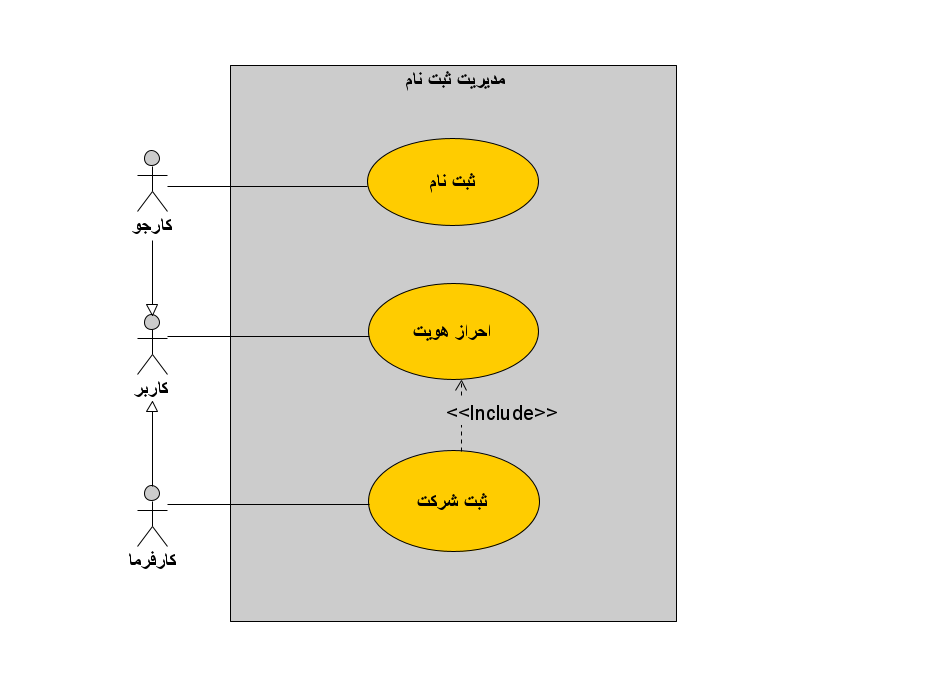
\includegraphics[width=\textwidth, height=12cm]{./images/1}
	\end{center}
\end{figure}

\begin{figure}[H]
	\caption{مورد کاربرد \arabic{figure}}
	\begin{center}
		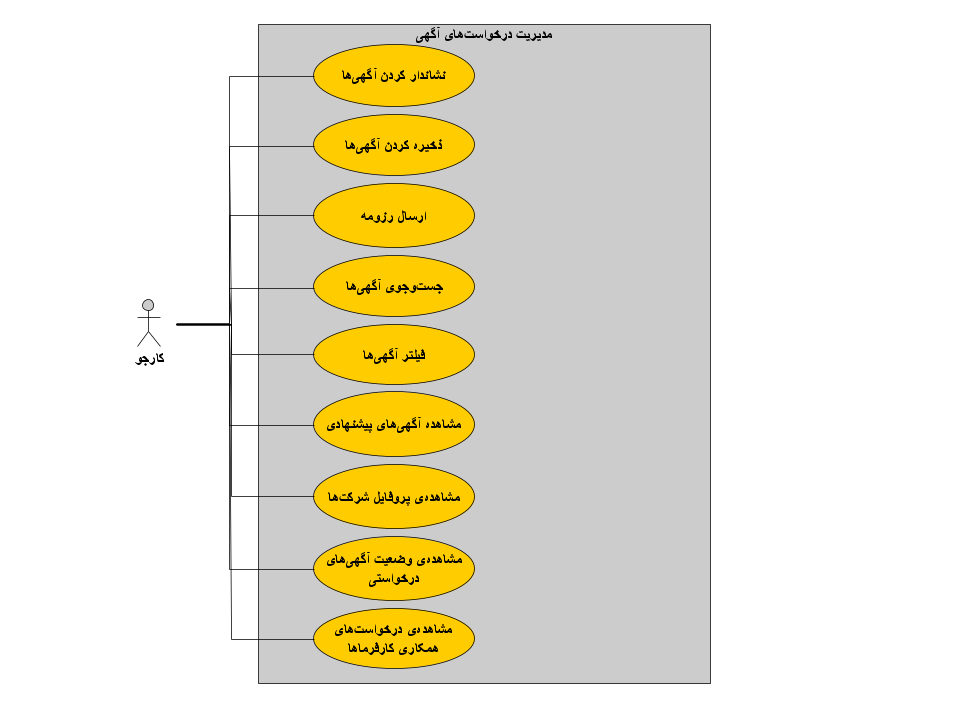
\includegraphics[width=\textwidth, height=12cm]{./images/2}
	\end{center}
\end{figure}

\begin{figure}[H]
	\caption{مورد کاربرد \arabic{figure}}
	\begin{center}
		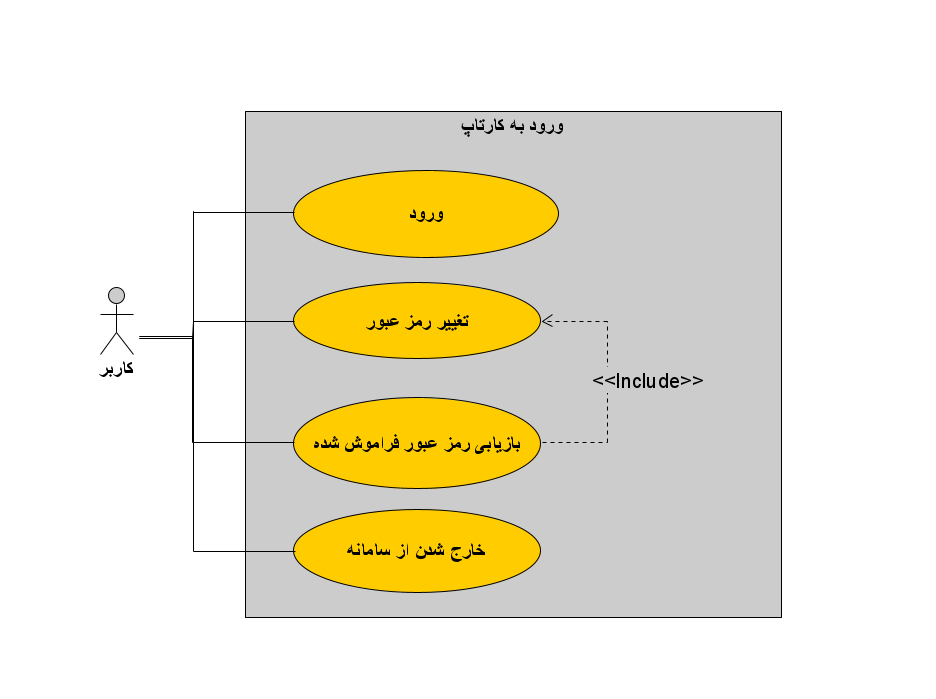
\includegraphics[width=\textwidth, height=12cm]{./images/3}
	\end{center}
\end{figure}

\begin{figure}[H]
	\caption{مورد کاربرد \arabic{figure}}
	\begin{center}
		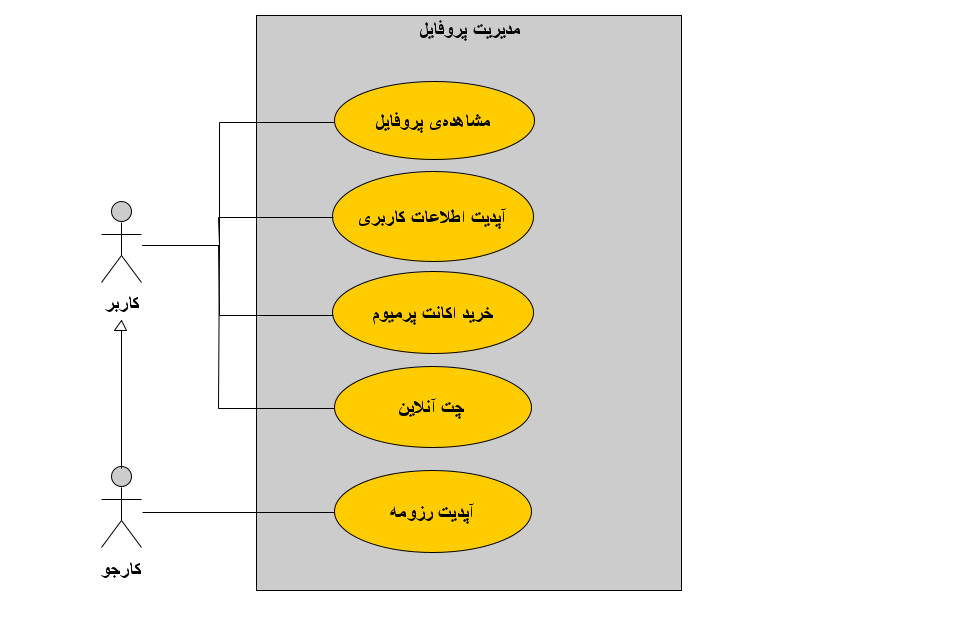
\includegraphics[width=\textwidth, height=12cm]{./images/4}
	\end{center}
\end{figure}

\begin{figure}[H]
	\caption{مورد کاربرد \arabic{figure}}
	\begin{center}
		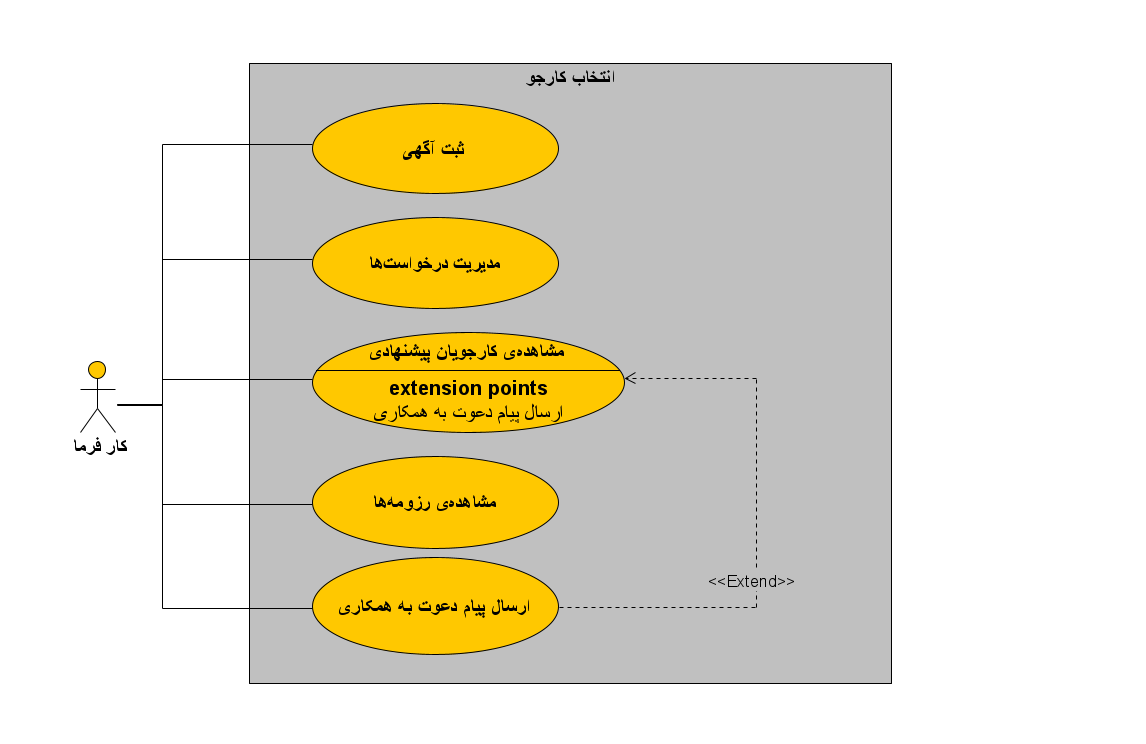
\includegraphics[width=\textwidth, height=12cm]{./images/5}
	\end{center}
\end{figure}

\section{بازبینی مورد کاربرد‌ها و نمودارها}		
در این گام مورد کاربرد‌ها، نیازمندی‌ها و ارتباط میان‌ آنها مجدداً بررسی شد و در قالب جدول \ref{table:review} تدوین گردید.

\begin{sidewaystable}
	\caption{جدول ردیابی موارد کاربرد}
	\label{table:review}
	\begin{adjustbox}{width=\textwidth}
		\begin{tabular}{|c|c|c|c|c|c|c|c|c|c|c|c|c|c|c|c|c|c|c|c|c|c|c|c|c|c|c|c|c|c|}
			\hline
			نیازمندی‌ها &
			اولویت &
			\uc{1} & 
			\uc{2} & 
			\uc{3} & 
			\uc{4} & 
			\uc{5} & 
			\uc{6} & 
			\uc{7} & 
			\uc{8} & 
			\uc{9} & 
			\uc{10} & 
			\uc{11} & 
			\uc{12} & 
			\uc{13} & 
			\uc{14} & 
			\uc{15} & 
			\uc{16} & 
			\uc{17} & 
			\uc{18} & 
			\uc{19} & 
			\uc{20} & 
			\uc{21} & 
			\uc{22} & 
			\uc{23} & 
			\uc{24} & 
			\uc{25} & 
			\uc{26} & 
			\uc{27} & 
			\uc{28} \\
			\hline
			
			\req{01} & 
			1 &
			& 
			& 
			& 
			& 
			& 
			& 
			& 
			& 
			& 
			& 
			& 
			\zstar & 
			& 
			& 
			& 
			& 
			& 
			& 
			& 
			& 
			&
			&
			&
			&
			&
			&
			&
			\\
			\hline
			\req{02} &
			1 &
			& 
			& 
			& 
			& 
			& 
			& 
			& 
			& 
			&
			\zstar &
			&
			&
			&
			& 
			& 
			& 
			\zstar & 
			& 
			& 
			& 
			& 
			& 
			& 
			& 
			& 
			&
			&
			\\
			\hline
			\req{03} &
			2 &
			& 
			& 
			& 
			& 
			& 
			& 
			& 
			& 
			\zstar & 
			&
			&
			&
			&
			&
			& 
			& 
			& 
			& 
			& 
			& 
			& 
			& 
			& 
			& 
			& 
			&
			&
			\\
			\hline
			\req{04} &
			1 &
			& 
			& 
			& 
			& 
			\zstar & 
			& 
			& 
			& 
			& 
			& 
			& 
			& 
			& 
			& 
			& 
			& 
			& 
			&
			&
			&
			&
			&
			& 
			& 
			& 
			&
			&
			\\
			\hline
			\req{05} &
			2 &
			& 
			& 
			& 
			& 
			& 
			\zstar & 
			& 
			& 
			& 
			& 
			& 
			& 
			& 
			& 
			& 
			& 
			& 
			& 
			&
			\zstar &
			&
			& & & & & & \\
			\hline
			\req{06} &
			1 &
			& 
			& 
			& 
			& 
			& 
			& 
			& 
			& 
			& 
			& 
			& 
			& 
			& 
			& 
			& 
			& 
			& 
			\zstar &
			&
			& 
			& 
			& & & & & & \\
			\hline
			\req{07} &
			1 &
			& 
			& 
			& 
			& 
			& 
			& 
			& 
			\zstar & 
			& 
			& 
			& 
			& 
			& 
			& 
			& 
			& 
			& 
			& 
			& 
			&
			&
			&
			&
			&
			&
			&
			\zstar &
			\\
			\hline
			\req{08} &
			1 &
			& 
			& 
			& 
			& 
			& 
			\zstar & 
			& 
			& 
			& 
			& 
			& 
			& 
			& 
			& 
			& 
			& 
			& 
			& 
			& 
			& & & & & & & & \\
			\hline
			\req{09} &
			1 &
			& 
			& 
			& 
			& 
			& 
			& 
			& 
			& 
			& 
			& 
			& 
			& 
			& 
			& 
			& 
			& 
			& 
			& 
			\zstar & 
			& & & & & & & &\\
			\hline
			\req{10} &
			2 &
			& 
			\zstar & 
			& 
			& 
			& 
			& 
			& 
			& 
			\zstar & 
			& 
			& 
			& 
			& 
			& 
			& 
			& 
			& 
			& 
			& 
			& & & & & & & &\\
			\hline
			\req{11} &
			2 &
			& 
			& 
			& 
			& 
			& 
			& 
			& 
			& 
			& 
			& 
			& 
			& 
			& 
			& 
			& 
			& 
			& 
			& 
			& 
			&
			&
			&
			\zstar &
			\zstar &
			&
			& &\\
			\hline
			\req{12} &
			3 &
			& 
			& 
			& 
			& 
			& 
			& 
			& 
			& 
			& 
			& 
			& 
			\zstar & 
			& 
			& 
			& 
			& 
			& 
			& 
			& 
			& & & & & & & &\\
			\hline
			\req{13} &
			3 &
			& 
			& 
			& 
			& 
			& 
			& 
			& 
			& 
			& 
			& 
			& 
			& 
			& 
			\zstar & 
			& 
			& 
			& 
			& 
			& 
			& & & & & & & &\\
			\hline
			\req{14} &
			2 &
			& 
			& 
			& 
			& 
			& 
			& 
			& 
			& 
			& 
			& 
			& 
			& 
			& 
			& 
			& 
			& 
			& 
			& 
			& 
			&
			&
			&
			&
			&
			& 
			\zstar & &\\
			\hline
			\req{15} &
			3 &
			& 
			& 
			& 
			& 
			& 
			\zstar & 
			& 
			& 
			& 
			& 
			& 
			& 
			& 
			& 
			& 
			& 
			& 
			& 
			& 
			& & & & & & & &\\
			\hline
			\req{16} &
			3 &
			& 
			& 
			& 
			& 
			& 
			\zstar & 
			& 
			& 
			& 
			& 
			& 
			& 
			& 
			& 
			& 
			& 
			& 
			& 
			& 
			& & & & & & & &\\
			\hline
			\req{17} &
			3 &
			& 
			& 
			& 
			& 
			& 
			& 
			& 
			& 
			& 
			& 
			& 
			& 
			& 
			& 
			\zstar & 
			& 
			& 
			& 
			& 
			& \zstar & & & & \zstar & & &\\
			\hline
			\req{18} &
			3 &
			& 
			& 
			& 
			& 
			& 
			& 
			& 
			& 
			& 
			& 
			& 
			& 
			& 
			\zstar & 
			& 
			& 
			& 
			& 
			& 
			& & & & & & & &\\
			\hline
			\req{19} &
			3 &
			& 
			& 
			& 
			& 
			\zstar & 
			& 
			& 
			& 
			& 
			& 
			\zstar & 
			& 
			\zstar & 
			& 
			& 
			& 
			& 
			& 
			& 
			&
			&
			\zstar &
			&
			&
			& & &\\
			\hline
			
			\req{20} &
			3 &
			& 
			& 
			& 
			& 
			& 
			& 
			\zstar & 
			& 
			& 
			& 
			& 
			& 
			& 
			& 
			& 
			& 
			& 
			& 
			& 
			& & & & & & & &\\
			\hline
			\req{21} &
			1 &
			\zstar & 
			& 
			& 
			& 
			& 
			& 
			& 
			& 
			& 
			& 
			& 
			& 
			& 
			& 
			& 
			& 
			& 
			& 
			& 
			& & & & & & & &\\
			\hline
			\req{22} &
			1 &
			& 
			& 
			& 
			& 
			& 
			& 
			& 
			& 
			& 
			& 
			& 
			\zstar & 
			& 
			& 
			& 
			& 
			& 
			& 
			& 
			& & & & & & & &\\
			\hline
			\req{23} &
			1 &
			& 
			\zstar & 
			& 
			\zstar & 
			& 
			& 
			& 
			& 
			& 
			& 
			& 
			& 
			& 
			& 
			& 
			& 
			& 
			& 
			& 
			& & & & & & & &\\
			\hline
			\req{24} &
			2 &
			& 
			& 
			& 
			& 
			& 
			& 
			& 
			& 
			& 
			& 
			& 
			& 
			& 
			& 
			& 
			\zstar & 
			& 
			& 
			& 
			& & & & & & & &\\
			\hline
			\req{25} &
			2 &
			& 
			& 
			& 
			& 
			& 
			& 
			& 
			& 
			& 
			& 
			& 
			& 
			& 
			& 
			& 
			& 
			& 
			& 
			& 
			& 
			&
			&
			&
			&
			&
			&
			&
			\zstar \\
			\hline
			\req{26} &
			2 &
			& 
			& 
			\zstar & 
			& 
			& 
			& 
			& 
			& 
			& 
			& 
			& 
			& 
			& 
			& 
			& 
			& 
			& 
			& 
			& 
			& & & & & & & & \\
			\hline
			اولویت مورد کاربرد‌ها &
			&
			1 & 
			1 & 
			2 & 
			1 & 
			1 & 
			1 & 
			3 & 
			1 & 
			2 & 
			1 & 
			3 & 
			1 & 
			3 & 
			3 & 
			3 & 
			2 & 
			1 & 
			1 & 
			1 & 
			2 & 3 & 3 & 2 & 2 & 3 & 2 & 1 & 2 \\
			\hline
			
		\end{tabular}
	\end{adjustbox}
\end{sidewaystable}


\section{تخصیص موارد کاربرد به تکرارها}		
موارد کاربرد بر اساس اولویت آنها در هر یک از سه تکرار برنامه‌ریزی شده پخش شده‌اند که در جدول \ref{table:repeat} قابل مشاهده است.

\begin{table}
	\caption{تخصیص موارد کاربرد به تکرار‌ها}
	\label{table:repeat}
	\begin{adjustbox}{width=\textwidth}
		\begin{tabular}{|c|c|c|c|c|c|c|}
			
			\hline
			مورد کاربر‌د‌ها &
			اولویت (۱-۳) &
			میزان تلاش (نفر در هفته) &
			وابسته به &	
			تکرار ۱ (۳ هفته) &
			تکرار ۲ (۳ هفته & 
			تکرار ۳ (۳ هفته) \\
			\hline
			\uc{1} &
			1 &
			2 &
			- &
			&
			&
			2 \\
			\hline
			\uc{2} &
			1 &
			3 &
			\uc{1} &
			1 &
			2 &
			\\
			\hline
			\uc{3} &
			2 &
			3 &
			\uc{2} &
			&
			3 &
			\\
			\hline
			\uc{4} &
			1 &
			2 &
			\uc{1} &
			2 &
			&
			\\
			\hline
			\uc{5} &
			1 &
			5 &
			\uc{2} &
			5 &
			&
			\\
			\hline
			\uc{6} &
			1 &
			5 &
			\uc{2} &
			3  &
			2 &
			\\
			\hline
			\uc{7} &
			3 &
			3 &
			\uc{2} &
			&
			&
			3 \\
			\hline
			\uc{8} &
			1 &
			3 &
			\uc{2} &
			3 &
			&
			\\
			\hline
			\uc{9} &
			2 &
			2 &
			\uc{2} &
			&
			2 &
			\\
			\hline
			\uc{10} &
			1 &
			1 &
			\uc{2} &
			&
			1 &
			\\
			\hline
			\uc{11} &
			3 &
			5 &
			\uc{2} &
			&
			&
			5 \\
			\hline
			\uc{12} &
			1 &
			2 &
			\uc{2} &
			&
			&
			1 \\
			\hline
			\uc{13} &
			3 &
			3 &
			\uc{2} &
			&
			&
			3 \\
			\hline
			\uc{14} &
			3 &
			2 &
			\uc{2} &
			&
			&
			2 \\
			\hline
			\uc{15} &
			3 &
			2 &
			\uc{2} &
			&
			&
			2 \\
			\hline
			\uc{16} &
			2 &
			2 &
			\uc{1} &
			&
			2 &
			\\
			\hline
			\uc{17} &
			1 &
			1 &
			\uc{2} &
			1 &
			&
			\\
			\hline
			\uc{18} &
			1 &
			3 &
			\uc{2} &
			3 &
			&
			\\
			\hline
			\uc{19} &
			1 &
			2 &
			\uc{2} &
			2 &
			& \\
			\hline
			
			\uc{20} &
			2 &
			1 &
			\uc{2} &
			&
			1 & \\
			\hline
			
			\uc{21} &
			3 &
			2 &
			\uc{2} &
			&
			& 2 \\
			\hline
			
			\uc{22} &
			3 &
			3 &
			\uc{2} &
			&
			& 3 \\
			\hline
			
			\uc{23} &
			2 &
			2 &
			\uc{2} &
			&
			2 & \\
			\hline
			
			\uc{24} &
			2 &
			2 &
			\uc{2} &
			&
			2 & \\
			\hline
			
			\uc{25} &
			3 &
			1 &
			\uc{2} &
			&
			& 1 \\
			\hline
			
			\uc{26} &
			2 &
			3 &
			\uc{2} &
			&
			3 & \\
			\hline
			
			\uc{27} &
			1 &
			1 &
			\uc{2} &
			1 &
			& \\
			\hline
			
			\uc{28} &
			2 &
			2 &
			\uc{2} &
			&
			2 & \\
			\hline
			
			\lr{Total Effort} &
			&
			68 &
			&
			26 &
			22 & 
			24 \\
			\hline
			
		\end{tabular} 
	\end{adjustbox}
\end{table}
\section{رعایت اصول چابکی}
تیم توسعه از طریق مصاحبه با کارجویان و کارفرمایان مختلف، مطالعه‌ی عملیات کسب‌وکار فعلی و همجنین جلسات اعضای گروه، توانست اطلاعات کافی و لازم جهت تدوین نیاز‌مندی‌ها و مورد کاربر‌د‌ها، بنا بر اولویت‌های مشتری را بدست آورد. در این بخش سعی شده است که مورد کاربرد‌ها در تکرار‌های منظم و با با فاصله زمانی مناسب در قالب یک تیم ۷ نفره، پیاده‌سازی شود.
